\documentclass[../main.tex]{subfiles}

\begin{document}

For testing purpose,we will use three UAM network topologies, first time presented in \cite{pelegrin-2023} and used and implemented in \cite{portoleau-2024}, and we can see a small example in Figure \ref{fig:topologies}.

\begin{figure}
\begin{subfigure}[b]{0.3\textwidth}
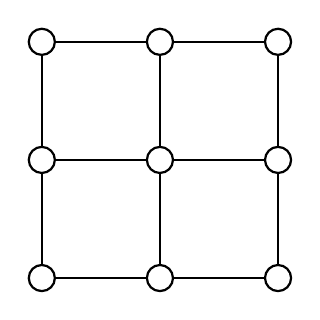
\begin{tikzpicture}[node distance={15mm}, thick, main/.style = {draw, circle}] 
\node[main] (1) {}; 
\node[main] (2) [right of=1] {}; 
\node[main] (3) [right of=2] {}; 
\node[main] (4) [below of=1] {}; 
\node[main] (5) [right of=4] {}; 
\node[main] (6) [right of=5] {}; 
\node[main] (7) [below of=4] {}; 
\node[main] (8) [right of=7] {}; 
\node[main] (9) [right of=8] {}; 

\draw (1) -- (2); 
\draw (2) -- (3);
\draw (1) -- (4); 
\draw (4) -- (5); 
\draw (5) -- (6); 
\draw (4) -- (7); 
\draw (7) -- (8); 
\draw (8) -- (9); 
\draw (2) -- (5); 
\draw (3) -- (6); 
\draw (5) -- (8); 
\draw (6) -- (9); 

\end{tikzpicture} 
\label{graph:grid}
\caption{Grid topology}
\end{subfigure}

\begin{subfigure}[b]{0.3\textwidth}
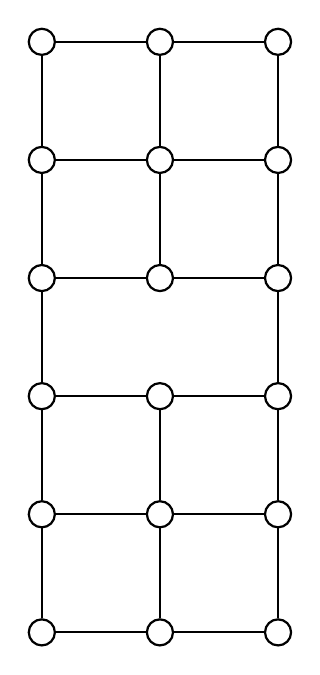
\begin{tikzpicture}[node distance={15mm}, thick, main/.style = {draw, circle}] 
\node[main] (1) {}; 
\node[main] (2) [right of=1] {}; 
\node[main] (3) [right of=2] {}; 
\node[main] (4) [below of=1] {}; 
\node[main] (5) [right of=4] {}; 
\node[main] (6) [right of=5] {}; 
\node[main] (7) [below of=4] {}; 
\node[main] (8) [right of=7] {}; 
\node[main] (9) [right of=8] {}; 

\node[main] (10) [below of=7] {}; 
\node[main] (11) [right of=10] {}; 
\node[main] (12) [right of=11] {}; 
\node[main] (13) [below of=10] {}; 
\node[main] (14) [right of=13] {}; 
\node[main] (15) [right of=14] {}; 
\node[main] (16) [below of=13] {}; 
\node[main] (17) [right of=16] {}; 
\node[main] (18) [right of=17] {}; 

\draw (1) -- (2); 
\draw (2) -- (3);
\draw (1) -- (4); 
\draw (4) -- (5); 
\draw (5) -- (6); 
\draw (4) -- (7); 
\draw (7) -- (8); 
\draw (8) -- (9); 
\draw (2) -- (5); 
\draw (3) -- (6); 
\draw (5) -- (8); 
\draw (6) -- (9); 

\draw (10) -- (11); 
\draw (11) -- (12);
\draw (13) -- (14); 
\draw (14) -- (15); 
\draw (16) -- (17); 
\draw (17) -- (18); 
\draw (10) -- (13); 
\draw (11) -- (14); 
\draw (12) -- (15); 
\draw (13) -- (16); 
\draw (14) -- (17); 
\draw (15) -- (18); 

\draw (7) -- (10); 
\draw (9) -- (12); 

\end{tikzpicture} 
\caption{Metroplex topology}
\end{subfigure}

\begin{subfigure}[b]{0.3\textwidth}
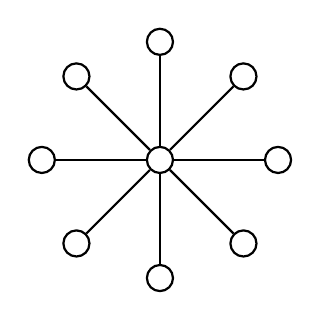
\begin{tikzpicture}[node distance={15mm}, thick, main/.style = {draw, circle}] 
\node[main] (1) {}; 
\node[main] (2) [above right of=1] {}; 
\node[main] (3) [right of=1] {}; 
\node[main] (4) [below right of=1] {}; 
\node[main] (5) [below of=1] {}; 
\node[main] (6) [below left of=1] {}; 
\node[main] (7) [left of=1] {}; 
\node[main] (8) [above left of=1] {}; 
\node[main] (9) [above of=1] {};

\draw (1) -- (2); 
\draw (1) -- (3);
\draw (1) -- (4); 
\draw (1) -- (5); 
\draw (1) -- (6); 
\draw (1) -- (7); 
\draw (1) -- (8); 
\draw (1) -- (9);
\end{tikzpicture} 
\caption{Airport topology}
\label{graph:airport}
\end{subfigure}

\caption{The different kinds of topologies}
\label{fig:topologies}
\end{figure}


\end{document}